
\begin{frame}
\frametitle{Occam's razor}
\begin{quote}
``Everything should be kept as simple as possible, but no simpler.''
\par \rightline{\tiny{\rm --- Einstein (allegedly)}}
\end{quote}
\vspace{0.25cm}
\begin{itemize}
\item Complex models (with many estimated parameters) usually explain training data better than simpler models.\par
\item Simpler models often generalise better to new data than nore complex models.\par
\end{itemize}
Need to find the model with the optimal bias/variance tradeoff.\par
\end{frame}

\begin{frame}
\frametitle{Bayesian model selection}
\emph{Real Bayesians don't cross-validate} (except when they need to).\par
\begin{align*}
P(M|\mathcal{D}) = \frac{p(\mathcal{D}|M) P(M)}{P(\mathcal{D})}\\
\end{align*}
The \emph{Bayes factor} allows the plausibility of two models ($M_1$ and $M_2$) to be compared:
\begin{align*}
K = \frac{p(\mathcal{D}|M_1)}{p(\mathcal{D}|M_2)} =
    \frac{\int_{\theta_{M_1}} p(\mathcal{D}|\theta_{M_1},M_1) p(\theta_{M_1}|M_1) d{\theta}_{M_1}}
         {\int_{\theta_{M_2}} p(\mathcal{D}|\theta_{M_2},M_2) p(\theta_{M_2}|M_2) d{\theta}_{M_2}}
\end{align*}
This is usually too costly in practice, so approximations are used.
\end{frame}

\begin{frame}
\frametitle{Model selection}
%\begin{quote}``In theory there is no difference between theory and practice. In practice there is.''
%\par \rightline{\tiny{\rm --- Yogi Berra}}
%\end{quote}
Some approximations/alternatives to the Bayesian approach:
\begin{itemize}
\item {\bf Laplace approximations}: find the MAP/ML solution and use a Gaussian approximation to the parameter uncertainty.
\item {\bf Minimum Message Length} (MML): an information theoretic approach.
\item {\bf Minimum Description Length} (MDL): an information theoretic approach based on how well the model compresses the data.
\item {\bf Akaike Information Criterion} (AIC): $-2\log p(\mathcal{D}|\theta) + 2 k$, where $k$ is the number of estimated parameters.
\item {\bf Bayesian Information Criterion} (BIC): $-2\log p(\mathcal{D}|\theta) + k\log q$, where $q$ is the number of observations.
%\item {\bf Deviance Information Criterion} (DIC) and others.
\end{itemize}
\end{frame}

\begin{frame}
\frametitle{Model selection by nested cross-validation}

Inner cross-validation loop used to evaluate model's performance on a
pre-defined grid of parameter and retain the best one.

\begin{itemize}
\item Safe, but costly.
\item Supported by some libraries (e.g. scikit-learn).
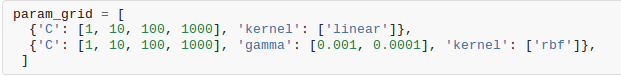
\includegraphics[width=\textwidth]{sklearn_material/grid}\\
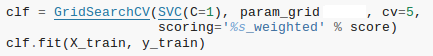
\includegraphics[width=.65\textwidth]{sklearn_material/grid_search}
\item Some estimators have path model, hence allow faster evaluation
  (e.g. LASSO).
\item Randomized techniques also exist, sometimes more efficient.
\item \textbf{Caveat:} inner cross-validation loop $\neq$ outer
  cross-validation loop for parameter evaluation
\end{itemize}
\end{frame} 

